
Bei der Entwicklung von StreamSwipe werden mehrere mögliche Einschränkungen der User betrachtet und entsprechend reagiert. Ziel ist es, dass sowohl der Kunde sowie der Anbieter maximal davon profitieren. Hierfür soll die App für ein möglichst großes Publikum zugänglich gemacht werden, jedoch auch sogenanntes Over-Engineering vermieden werden, da zu viele Funktionen eine App unübersichtlich, teuer und langsamer werden lassen.\\

\noindent
Allgemein wird Leserlichkeit durch große Schriftgrößen, hohe Farbkontraste, große Schaltflächen oder universelles Design erreicht. Alleine in Deutschland tragen 44,5 Millionen Menschen regelmäßig eine Brille oder Kontaktlinsen und benötigen somit Sehhilfen \cite{sehhilfen}. Unterstützung auf Seiten der App kann hierfür durch vergrößerbaren Text geschehen. Da aber davon ausgegangen werden kann, dass Personen, die sich auf Sehhilfen verlassen, bereits eine Brille oder Kontaktlinsen besitzen, wird die Textgröße vorerst nicht variabel gehalten. Außerdem gibt es bei Android- und Apple-Smartphones bereits eingebaute Vergrößerungsfeatures, die Bildausschnitte vergrößert darstellen können. Aus diesem Grund wird in diesem Projekt kein Fokus auf dieses Feature gelegt. \\
Farbblindheit kann jedoch in vielen Formen auftreten. Um der bekannten Farbfehlsicht entgegenzuwirken, werden Farben aus Problembereichen wie Rot und Grün nicht nebeneinander benutzt. Allgemein wird ein schlichtes Design gewählt und Farben nur zu Akzentuierung und als Stilmittel benutzt, statt als Informationsträger wie beispielsweise in den Abbildungen \ref{fig:bf-beispiel_a} erkennbar ist.  Geringe Sehschärfe durch Achromatopsie kann wie weiter oben beschrieben umgangen werden.\\


\begin{figure}[tbt]
	\begin{subfigure}{0.5\textwidth}
	\centering
	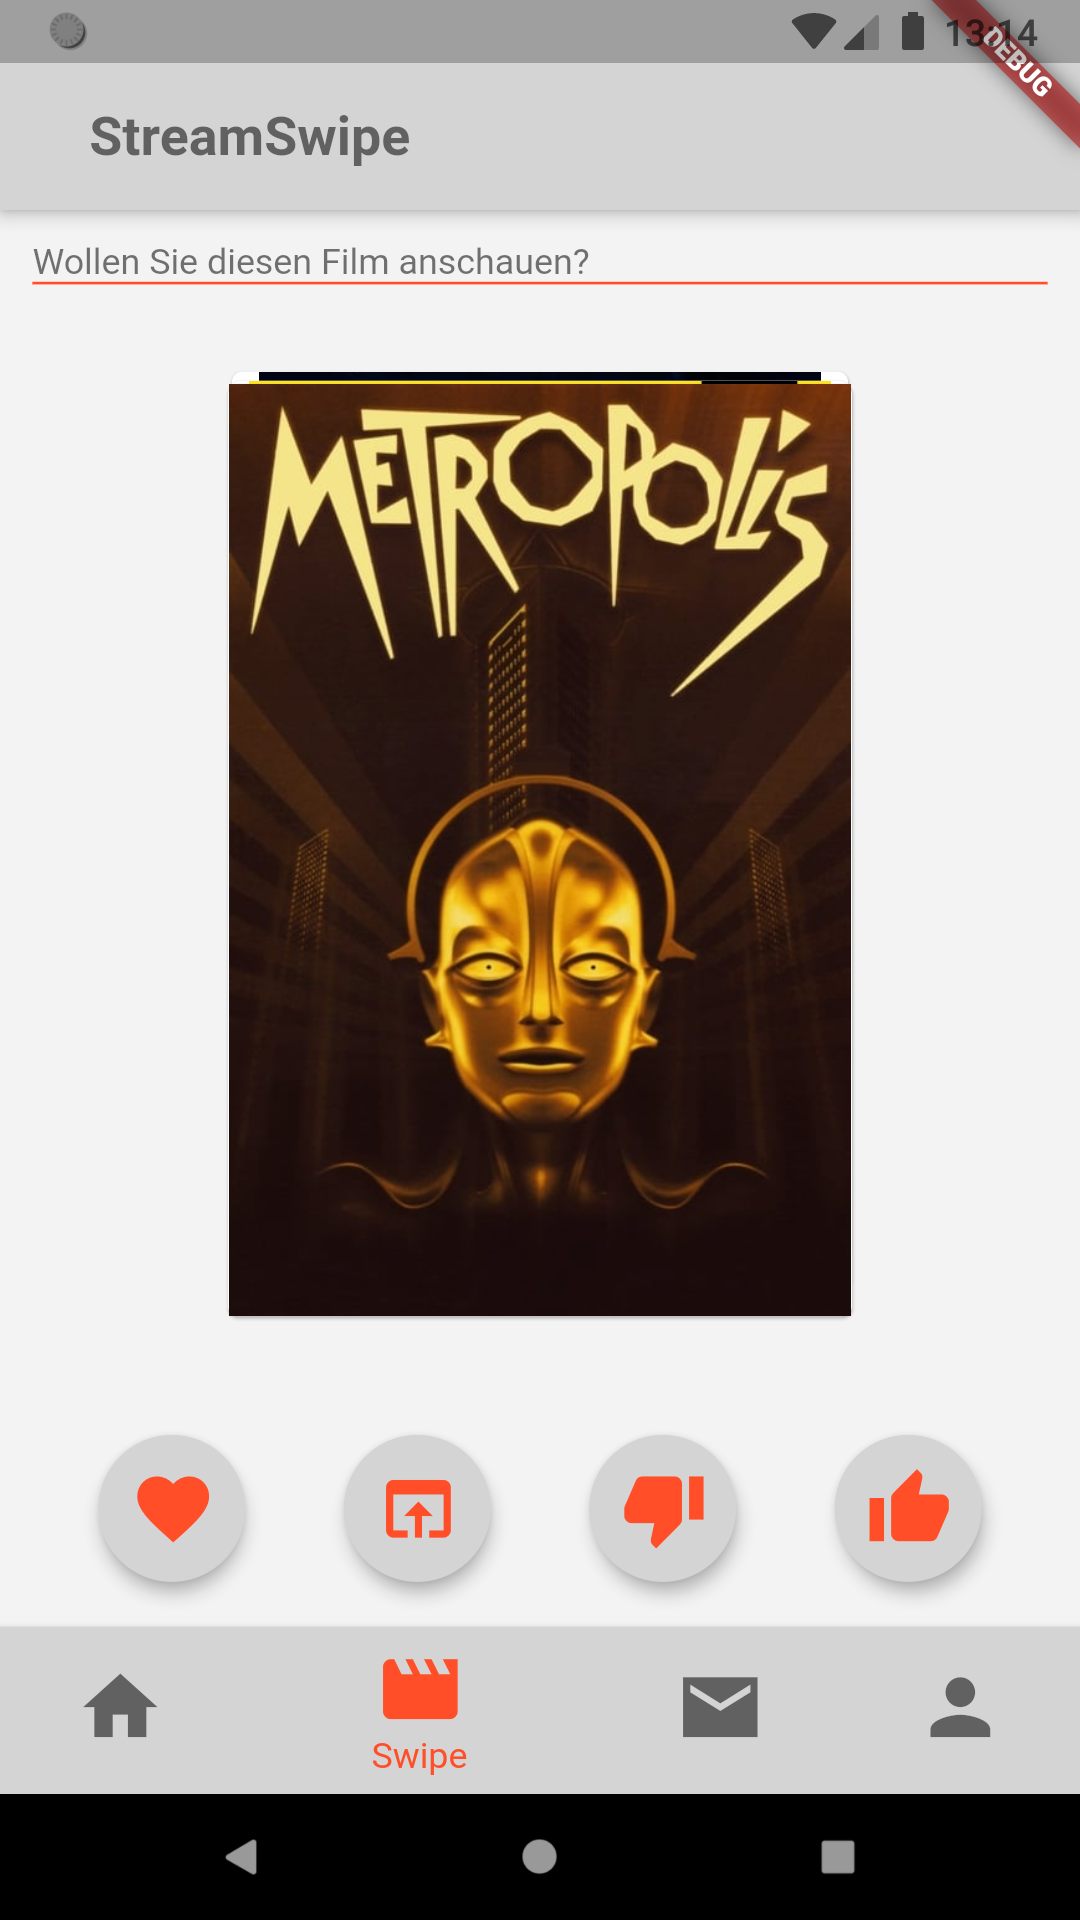
\includegraphics[scale=0.15]{Barrierefreiheit/images/bsp-swipe.png}
	\caption{}
	\label{fig:bf-beispiel_a}
	\end{subfigure}
	\begin{subfigure}{0.5\textwidth}
	\centering
	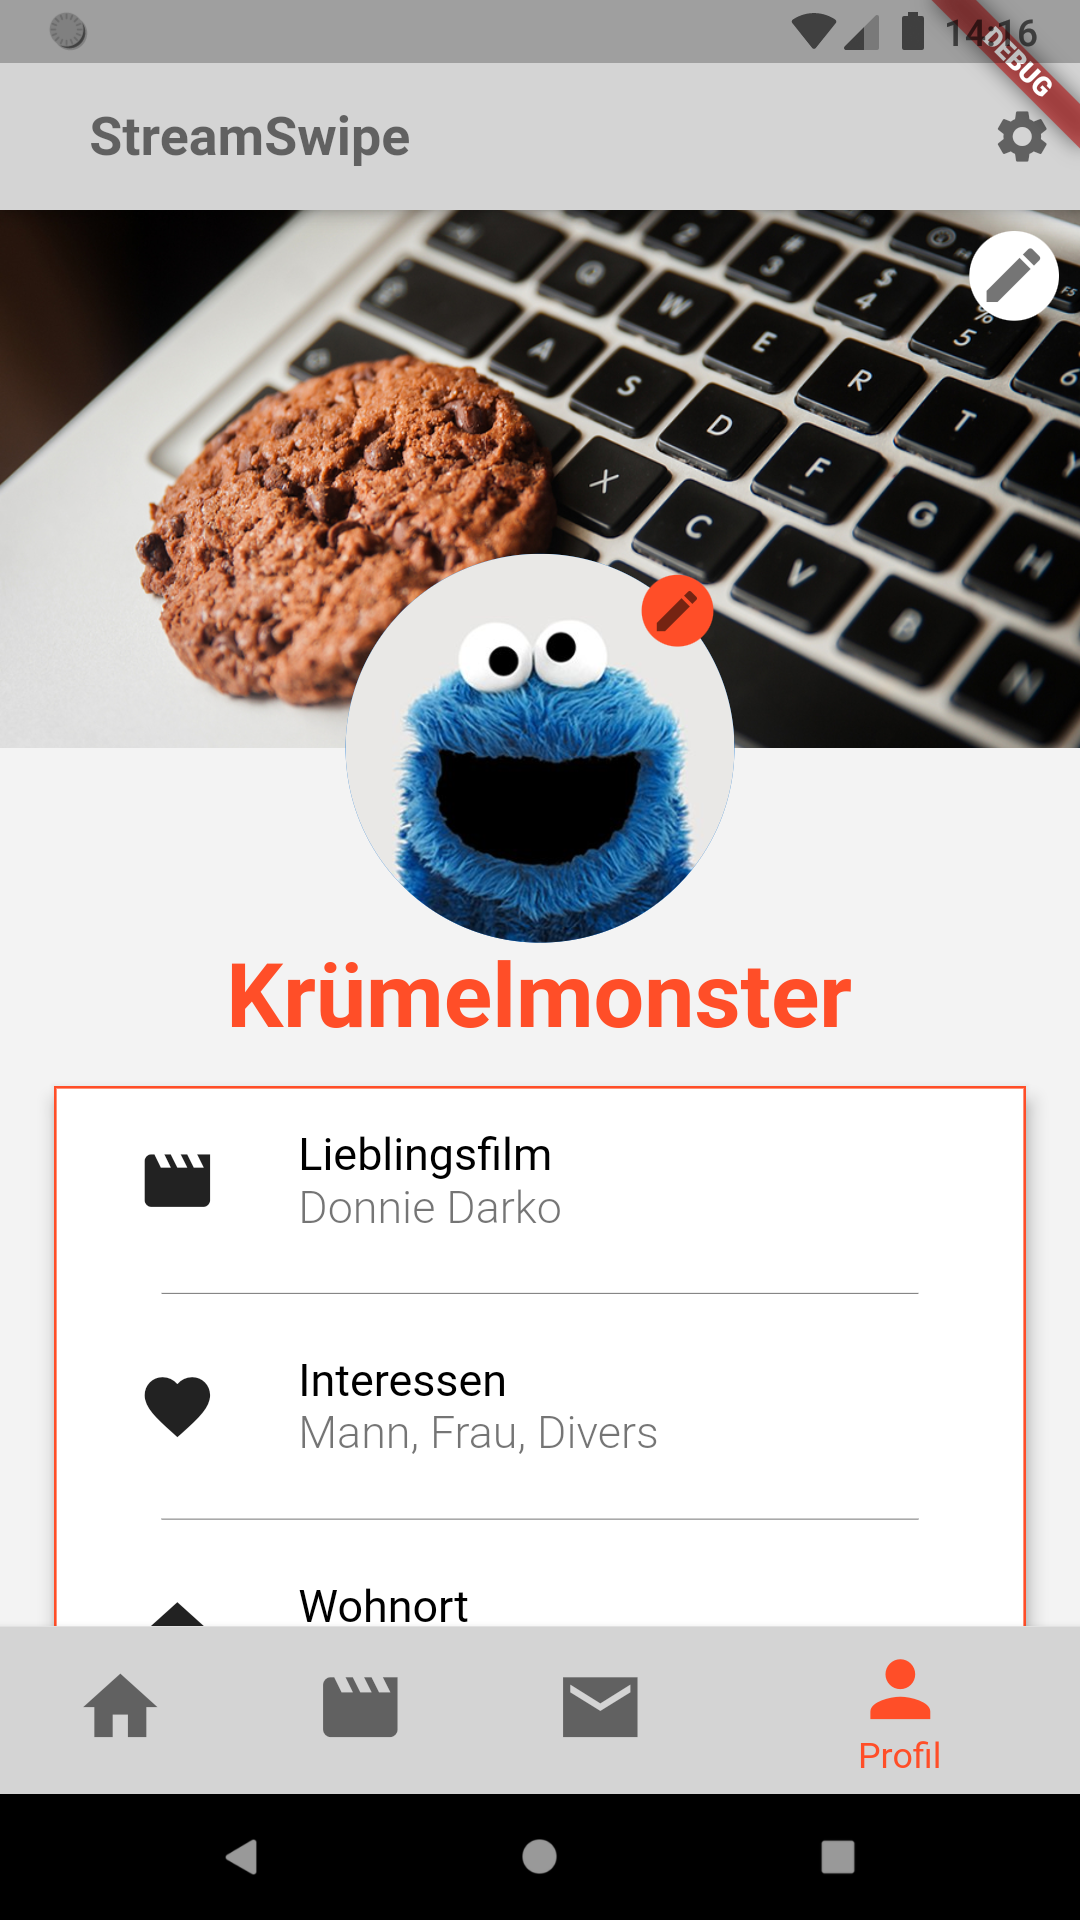
\includegraphics[scale=0.15]{Barrierefreiheit/images/bsp-profil.png}
	\caption{}
	\label{fig:bf-beispiel_b}
	\end{subfigure}
\caption{Screenshots aus der App StreamSwipe als Beispiele zu (a) schlichtem Design, bei dem farbige Akzente nicht der Informationenübertragung dienen um die Zugänglichkeit für farbblinde Menschen zu verbessern und für einen Icon in (b), welcher sonst durch sehgeschädigte Menschen nicht wahrnehmbar ist, wird exemplarisch eine Semantik implementiert.}
\label{fig:BF-Beispiele}
\end{figure}


\noindent
Ist die Sehkraft noch weiter eingeschränkt oder gar nicht mehr vorhanden, werden Semantiken eingesetzt. Hierbei erhält jedes Element auf dem Bildschirm eine Beschreibung, die vorgelesen werden kann. Bei Zahlen und Texten werden diese vorgelesen, sofern keine weitere Information hinterlegt ist. Besonders hilfreich ist dies jedoch bei Abbildungen. Ausgeführt wird das Auslesen von einem Screenreader. Mobile Geräte haben diese Funktion bereits standardmäßig eingebaut (VoiceOver bei Apple und TalkBack bei Android) und wandeln die Semantiken mittels Sprachsynthese in akustische Signale um. Bei Desktopanwendungen wie z.B. JAWS für Windows können diese Informationen zusätzlich auch durch eine Braillezeile wiedergegeben werden.\\
Bei Flutter ist das Hinzufügen von Semantiken bereits eingebaut. Hierfür kann ein String dem jeweiligen Bereich zugeordnet werden. In Beispiel \ref{lst:semantics} ist hierfür der Code des Buttons, der zu den Einstellungen führt. In Abbildung \ref{fig:bf-beispiel_b} ist dieser Button ganz rechts oben im Eck zu sehen.\\
Der GestureDetector erkennt Interaktionen mit dem Touchscreen, wobei hier nur auf Antippen reagieren soll, deshalb die Funktion onTap:()$\{\}$, die auf den Einstellungsbildschirm leitet. Diese Implementierung ist hier aber nicht von Relevanz und wird übersprungen. In dem GestureDetector ist ein Icon eingebettet, von der Form \textit{Settings}, was einem Zahnrad entspricht. Dieses Icon erhält eine Farbe und anschließend eine Semantik aus allem was in den Anführungszeichen steht. Ein Screenreader kann AE erkennen und ihn als den Umlaut Ä aussprechen. \\
So wird im kompletten Programm für jedes relevante Element vorgegangen. Teilweise  müssen den Semantiken Variablen übergeben werden, da sich die vorzulesende Information ändert wie beispielsweise bei den Filmtiteln.
    
\begin{lstlisting}[caption=Codeausschnitt in Dart von einem Button mit Semantiken.,label=lst:semantics]
GestureDetector(
  onTap: () {
     ...
  },
  child: Icon(
    Icons.settings,
    color: Provider.of(context).colors.textSmall,
    semanticLabel: "Einstellungen. Zum Auswaehlen doppeltippen.",
  )
),
\end{lstlisting}

\noindent
Bei einer sauberen Implementierung wird auf diese Weise vorgegangen und eine bereits vorhandene Funktion verwendet. Dies vereinfacht nicht nur die Leserlichkeit des Codes, sondern bietet auch die höchste Modularität, da hierbei normalerweise standardisierte Schnittstellen für Betriebssysteme oder andere Anwendungen verwendet werden. In diesem Fall  müssen die Screenreader von Android und Apple damit arbeiten können.\\

\noindent 
Um für Personen mit eingeschränktem Hörvermögen oder vollständiger Gehörlosigkeit die App zugänglich zu machen, wird auf akustisches Feedback als notwendige Infor"-mations"-über"-tragung verzichtet. Innerhalb der App werden keine Geräusche erzeugt, außer der oben beschriebenen Funktion der Semantiken. Beim Erhalten einer neuen Nachricht oder eines neuen Matches kann weiterhin optional eine akustische Benachrichtigung erhalten werden. Hierbei wird die betriebssystemeigene Funktion übernommen, sodass in der App keine neuen Einstellungen vorgenommen werden müssen.\\

\noindent
Auch feinmotorische Einschränkungen werden versucht zu umgehen. Die Navigation und die Filmbewertung in StreamSwipe können durch großflächige Wischbewegungen ausgeführt werden. Wo diese Lösung nicht möglich ist, werden verhältnismäßig große Buttons eingesetzt. Lediglich beim Registrieren und Einloggen werden feine Bewegungen erfordert. Hierbei öffnet sich allerdings die als Standard eingestellte digitale Tastatur, die in vielen Fällen eine Spracheingabe besitzt, sodass die sehr kleinen Tasten nicht benutzt werden müssen.\\

%TODO Diesen Satz evtl. ganz ans Ende ins Fazit
\noindent
Sollte sich in Zukunft jedoch Kritik in Form von negativen Nutzerbewertungen herauskristallisieren, kann eines der noch nicht implementierten Features über ein Update nachgerüstet werden.